\RequirePackage{currfile}
\documentclass[12pt]{beamer}
\usepackage[utf8]{inputenc}
\usepackage[spanish]{babel}
\usepackage{standalone}
\usepackage{color}
\usepackage{siunitx}
\usepackage{hyperref}
%\hypersetup{colorlinks,linkcolor=,urlcolor=blue}
%\hypersetup{colorlinks,urlcolor=blue}
\usepackage{xcolor,soul}
\usepackage{etoolbox}
\usepackage{amsmath}
\usepackage{amsthm}
\usepackage{physics}
\usepackage{multicol}
\usepackage{bookmark}
\usepackage{longtable}
\usepackage{listings}
\usepackage{graphicx}
\usepackage{tikz}
\usetikzlibrary{patterns, matrix, backgrounds, decorations,shapes, arrows.meta}
\usepackage[autostyle,spanish=mexican]{csquotes}
\usepackage[os=win]{menukeys}
\usepackage{pifont}
\usepackage{pbox}
\usepackage{caption}
\captionsetup{font=scriptsize,labelfont=scriptsize}
%\usepackage[sfdefault]{roboto}  %% Option 'sfdefault' only if the base font of the document is to be sans serif

%Sección de definición de colores
\definecolor{ao}{rgb}{0.0, 0.5, 0.0}
\definecolor{bisque}{rgb}{1.0, 0.89, 0.77}
\definecolor{amber}{rgb}{1.0, 0.75, 0.0}
\definecolor{armygreen}{rgb}{0.29, 0.33, 0.13}
\definecolor{alizarin}{rgb}{0.82, 0.1, 0.26}
\definecolor{cadetblue}{rgb}{0.37, 0.62, 0.63}
\definecolor{deepblue}{rgb}{0,0,0.5}
\definecolor{brown}{rgb}{0.59, 0.29, 0.0}
\definecolor{OliveGreen}{rgb}{0,0.25,0}


\usefonttheme[onlymath]{serif}
%Sección de definición de nuevos comandos

\newcommand*{\TitleParbox}[1]{\parbox[c]{1.75cm}{\raggedright #1}}%
\newcommand{\python}{\texttt{python}}
\newcommand{\textoazul}[1]{\textcolor{blue}{#1}}
\newcommand{\azulfuerte}[1]{\textcolor{blue}{\textbf{#1}}}
\newcommand{\funcionazul}[1]{\textcolor{blue}{\textbf{\texttt{#1}}}}
\newcommand{\ptilde}[1]{\ensuremath{{#1}^{\prime}}}
\newcommand{\stilde}[1]{\ensuremath{{#1}^{\prime \prime}}}
\newcommand{\ttilde}[1]{\ensuremath{{#1}^{\prime \prime \prime}}}
\newcommand{\ntilde}[2]{\ensuremath{{#1}^{(#2)}}}
\renewcommand{\arraystretch}{1.5}

\newcounter{saveenumi}
\newcommand{\seti}{\setcounter{saveenumi}{\value{enumi}}}
\newcommand{\conti}{\setcounter{enumi}{\value{saveenumi}}}
\renewcommand{\rmdefault}{cmr}% cmr = Computer Modern Roman

\linespread{1.5}

\usefonttheme{professionalfonts}
%\usefonttheme{serif}
\DeclareGraphicsExtensions{.pdf,.png,.jpg}


%Sección para el tema de beamer, con el theme, usercolortheme y sección de footers
\mode<presentation>
{
  \usetheme{Warsaw}
  
  %\useoutertheme{infolines}
  \useoutertheme{default}
  \usecolortheme{spruce}
  \setbeamercovered{invisible}
  % or whatever (possibly just delete it)
  \setbeamertemplate{section in toc}[sections numbered]
  \setbeamertemplate{subsection in toc}[subsections numbered]
  \setbeamertemplate{subsection in toc}{\leavevmode\leftskip=3.2em\rlap{\hskip-2em\inserttocsectionnumber.\inserttocsubsectionnumber}\inserttocsubsection\par}
  \setbeamercolor{section in toc}{fg=blue}
  \setbeamercolor{subsection in toc}{fg=blue}
  \setbeamercolor{frametitle}{fg=blue}
  \setbeamertemplate{caption}[numbered]

  \setbeamertemplate{footline}
  \beamertemplatenavigationsymbolsempty
  \setbeamertemplate{headline}{}
}

\makeatletter
\setbeamercolor{section in foot}{bg=gray!30, fg=black!90!orange}
\setbeamercolor{subsection in foot}{bg=blue!30!yellow, fg=red}
\setbeamertemplate{footline}
{
  \leavevmode%
  \hbox{%
  \begin{beamercolorbox}[wd=.333333\paperwidth,ht=2.25ex,dp=1ex,center]{section in foot}%
    \usebeamerfont{section in foot} \insertsection
  \end{beamercolorbox}}%
  \begin{beamercolorbox}[wd=.333333\paperwidth,ht=2.25ex,dp=1ex,center]{subsection in foot}%
    \usebeamerfont{subsection in foot}  \insertsubsection
  \end{beamercolorbox}%
  \begin{beamercolorbox}[wd=.333333\paperwidth,ht=2.25ex,dp=1ex,right]{date in head/foot}%
    \usebeamerfont{date in head/foot} \insertshortdate{} \hspace*{2em}
    \insertframenumber{} / \inserttotalframenumber \hspace*{2ex} 
  \end{beamercolorbox}}%
  \vskip0pt%
\makeatother  

\makeatletter
\patchcmd{\beamer@sectionintoc}
  {\vfill}
  {\vskip\itemsep}
  {}
  {}
\makeatother


\title{\large{Sistema de coordenadas parabólicas \\ Ejercicio completo}}
\subtitle{Tema 1 - La física y la geometría}
\author{}
\date{\today}
\institute{Facultad de Ciencias - UNAM}
\titlegraphic{
\includegraphics[width=1.75cm]{../Imagenes/escudo-facultad-ciencias}\hspace*{4.75cm}~%
   
\includegraphics[width=1.75cm]{../Imagenes/escudo-unam}
}
\setbeamertemplate{navigation symbols}{}
\begin{document}
\maketitle
\fontsize{14}{14}\selectfont
\spanishdecimal{.}
\section*{Contenido}
\frame[allowframebreaks]{\tableofcontents[currentsection, hideallsubsections]}
\section{Coordenadas curvilíneas ortogonales}
\frame[allowframebreaks]{\tableofcontents[currentsection, hideothersubsections]}
\subsection{Objetivos}
\begin{frame}
\frametitle{Objetivos}
A partir del sistema de coordenadas parabólico:
\setbeamercolor{item projected}{bg=blue!70!black,fg=yellow}
\setbeamertemplate{enumerate items}[circle]
\begin{enumerate}[<+->]
\item Se describirán las superficies coordenadas.
\item Se expresará un vector de posición.
\item Se demostrará que el sistema coordenado es ortogonal
\seti
\end{enumerate}
\end{frame}
\begin{frame}
\frametitle{Objetivos}
\setbeamercolor{item projected}{bg=blue!70!black,fg=yellow}
\setbeamertemplate{enumerate items}[circle]
\begin{enumerate}[<+->]
\conti
\item Se obtendrán los factores de escala.
\item Se determinará la base ortonormal.
\item Se calculará el elemento de volumen.
\seti
\end{enumerate}
\end{frame}
\begin{frame}
\frametitle{Objetivos}
\setbeamercolor{item projected}{bg=blue!70!black,fg=yellow}
\setbeamertemplate{enumerate items}[circle]
\begin{enumerate}[<+->]
\conti
\item Se obtendrán los operadores diferenciales.
\item Se calculará la velocidad de una partícula.
\item Se calculará la aceleración de una partícula.
\item Se calcularán los símbolos de Christtofel.
\end{enumerate}
\end{frame}
\section{Reglas de transformación}
\frame[allowframebreaks]{\tableofcontents[currentsection, hideothersubsections]}
\subsection{Coordenadas \texorpdfstring{$(u, v, \phi)$}{(u, v, f)}}
\begin{frame}
\frametitle{Reglas de transformación}
Las reglas de transformación para el sistema coordenado parabólico son:
\begin{align}
\begin{aligned}
x &= u \, v \, \cos \phi \\[0.5em]
y &= u \, v \, \sin \phi \\[0.5em]
z &= \dfrac{1}{2} (u^{2} + v^{2})
\end{aligned}
\label{eq:ecuacion_01}
\end{align}
\end{frame}
\section{Superficies coordenadas}
\frame[allowframebreaks]{\tableofcontents[currentsection, hideothersubsections]}
\subsection{Descripción}
\begin{frame}
\frametitle{Superficies coordenadas}
Recordemos que para determinar las superficies coordenadas del sistema coordenado de estudio, debemos de considerar cada una de las tres variables $(u, v, \phi)$ como constante, de esta manera podremos identificar las superficies constantes.
\end{frame}
\begin{frame}
\frametitle{Eje de traslación}
Considerando que el eje $z$ es un eje de translación para este sistema coordenado, haremos previamente una suma de cuadrados.
\end{frame}
\begin{frame}
\frametitle{Expresión para $x^{2}+ y^{2}$}
De la regla de transformación (\ref{eq:ecuacion_01}), al sumar el cuadrado de $x$ e $y$ tenemos que:
\begin{align*}
x^{2} + y^{2} &= (u \, v \, \cos \phi)^{2} + (u \, v \, \sin \phi)^{2} = \\[0.5em]
&= (u^{2} \, v^{2} \, \cos^{2} \phi) + (u^{2} \, v^{2} \, \sin^{2} \phi) = \\[0.5em]
&= (u^{2} \, v^{2}) (\cos^{2} \phi + \sin^{2} \phi) = \\[0.5em]
&= u^{2} \, v^{2}
\end{align*}
Entonces:
\end{frame}
\begin{frame}
\frametitle{Expresión para $x^{2}+ y^{2}$}
Se tiene que
\begin{align*}
x^{2}+ y^{2} = u^{2} \, v^{2}
\end{align*}
\pause
Para $v \neq 0$:
\begin{align*}
u^{2} = \dfrac{x^{2}+ y^{2}}{v^{2}}
\end{align*}
\pause
De la misma forma que, para $u \neq 0$:
\begin{align*}
v^{2} = \dfrac{x^{2}+ y^{2}}{u^{2}}
\end{align*}
\end{frame}
\begin{frame}
\frametitle{La coordenada $z$}
La coordenada $z$ queda definida por:
\begin{align}
2 \, z = \dfrac{x^{2}+ y^{2}}{u^{2}} - u^{2}
\label{eq:ecuacion_02}
\end{align}
y por
\begin{align}
2 \, z = - \left( \dfrac{x^{2}+ y^{2}}{v^{2}} \right) + v^{2}
\label{eq:ecuacion_03}
\end{align}
\end{frame}
\begin{frame}
\frametitle{Superficies coordenadas}
De la ec. (\ref{eq:ecuacion_02}) tenemos un paraboloide de revolución que abre en la dirección $z > 0$.
\\
\bigskip
Mientras que de la ec. (\ref{eq:ecuacion_03}), el paraboloide de revolución, abre en la dirección $z < 0$.
\end{frame}

\begin{frame}
\frametitle{Superficies coordenadas}
Al tomar el cociente $\dfrac{y}{x}$:
\begin{align*}
\dfrac{y}{x} = \tan \phi \hspace{1cm} \Longrightarrow \hspace{1cm} y = x \, \tan \phi
\end{align*}
Tenemos una familia de medios planos.
\\
\bigskip
En la siguiente figura (\ref{fig:figura_parabolica_3d}) aprecian las superficies coordenadas para este sistema parabólico.
\end{frame}
\begin{frame}
\frametitle{Superficies coordenadas}
\begin{figure}[H]
    \centering
    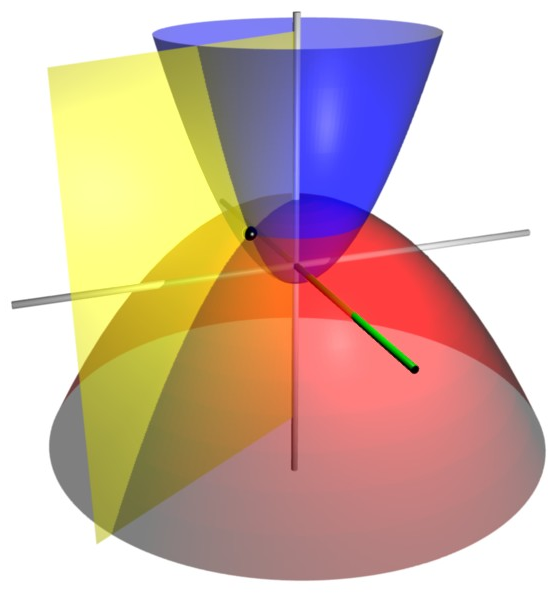
\includegraphics[scale=0.25]{Imagenes/Parabolic_coordinates_3D.png}
    \caption{Superficies coordenadas del sistema parabólico.}
    \label{fig:figura_parabolica_3d}
\end{figure}
\end{frame}
\section{Vector de posición}
\frame[allowframebreaks]{\tableofcontents[currentsection, hideothersubsections]}
\subsection{Un vector en el sistema}
\begin{frame}
\frametitle{Expresar un vector en el sistema}
Un vector $\va{r}$ queda determinado en el sistema cartesiano por:
\begin{align*}
\va{r} = x \, \vu{i} + y \, \vu{j} + z \, \vu{k}
\end{align*}
\pause
Con las reglas de transformación (\ref{eq:ecuacion_01}), tenemos:
\begin{align*}
\va{r} = u \, v \, \cos \phi \, \vu{i} + u \, v \, \sin \phi \, \vu{j} + \dfrac{1}{2} (u^{2} - v^{2}) \, \vu{k}
\end{align*}
\end{frame}
\begin{frame}
\frametitle{Derivadas parciales}
Vamos a requerir de las derivadas parciales del vector con respecto a $(u, v, \phi)$, por lo que es buen momento para calcularlas.
\end{frame}
\begin{frame}
\frametitle{Derivadas parciales}
\begin{align}
\begin{aligned}
\pdv{\va{r}}{u} &= v \, \cos \phi \vu{i} + v \, \sin \phi \, \vu{j} + u \, \vu{k} \\[0.5em]
\pdv{\va{r}}{v} &= u \, \cos \phi \vu{i} + u \, \sin \phi \, \vu{j} - v \, \vu{k} \\[0.5em]
\pdv{\va{r}}{\phi} &= - u \, v \, \sin \phi \vu{i} + u \, v \, \cos \phi
\end{aligned}
\label{eq:ecuacion_04}
\end{align}
\end{frame}
\section{Ortogonalidad del sistema}
\frame[allowframebreaks]{\tableofcontents[currentsection, hideothersubsections]}
\subsection{Demostración}
\begin{frame}
\frametitle{Ortogonalidad del sistema}
Para demostrar que el sistema es ortogonal, basta con calcular el producto punto de las derivadas parciales (\ref{eq:ecuacion_04}) y comprobar que el resultado es nulo.
\end{frame}
\begin{frame}
\frametitle{Calculando el producto punto}
\begin{align*}
\pdv{\va{r}}{u} \cdot \pdv{\va{r}}{v} &= u \, v \, \cos^{2} \phi + u \, v \sin^{2} \phi - u \, v = \\[0.5em]
&= u \, v \left( cos^{2} \phi + \sin^{2} \phi \right) - u\, v = \\[0.5em]
&= u \, v - u \, v \\[0.5em]
&= 0
\end{align*}
\end{frame}
\begin{frame}
\frametitle{Producto punto}
\begin{align*}
\pdv{\va{r}}{v} \cdot \pdv{\va{r}}{\phi} &= - u^{2} \, v \,  \cos \phi \sin \phi + u^{2} \, v \ ,\cos \phi \sin \phi = 0 \\[1em]
\pdv{\va{r}}{u} \cdot \pdv{\va{r}}{\phi} &= - u \, v^{2} \, \cos \phi \sin \phi + u \, v^{2} \, \cos \phi \sin \phi = 0
\end{align*}
\end{frame}
\begin{frame}
\frametitle{Ortogonalidad demostrada}
Al haber obtenido que el producto punto entre las derivadas parciales es nulo, se demuestra que el sistema es ortogonal.
\\
\bigskip
En caso de que algún valor del producto no fuese nulo, el sistema no es ortogonal.
\end{frame}
\section{Factores de escala}
\frame[allowframebreaks]{\tableofcontents[currentsection, hideothersubsections]}
\subsection{Obtención}
\begin{frame}
\frametitle{Calculando los factores de escala}
Para obtener los factores de escala del sistema coordenado parabólico, ocupamos la expresión:
\begin{align*}
h_{i} = \abs{\pdv{\va{r}}{u_{i}}}
\end{align*}
de tal manera que:
\end{frame}
\begin{frame}
\frametitle{Calculando los factores de escala}
\begin{align*}
h_{u} &= \sqrt{\left(\pdv{x}{u}\right)^{2} + \left(\pdv{y}{u}\right)^{2} + \left(\pdv{z}{u}\right)^{2}} \\[1em]
h_{v} &= \sqrt{\left(\pdv{x}{v}\right)^{2} + \left(\pdv{y}{v}\right)^{2} + \left(\pdv{z}{v}\right)^{2}} \\[1em]
h_{\phi} &= \sqrt{\left(\pdv{x}{\phi}\right)^{2} + \left(\pdv{y}{\phi}\right)^{2} + \left(\pdv{z}{\phi}\right)^{2}}
\end{align*}
\end{frame}
\begin{frame}
\frametitle{Las derivadas}
El cálculo de las derivadas parciales es inmediato:
\begin{table}
\centering
\fontsize{12}{12}\selectfont
\begin{tabular}{l l l}
$\displaystyle \pdv{x}{u} = v \, \cos \phi$ & $\displaystyle \pdv{y}{u} = v \, \sin \phi$ & $\displaystyle \pdv{z}{u} = u$ \\[0.5em]
$\displaystyle \pdv{x}{v} = u \, \cos \phi$ & $\displaystyle \pdv{y}{v} = u \, \sin \phi$ & $\displaystyle \pdv{z}{v} = - v$ \\[0.5em]
$\displaystyle \pdv{x}{\phi} = - u \, v \, \sin \phi$ & $\displaystyle \pdv{y}{\phi} = u \, v \, \cos \phi$ & $\displaystyle \pdv{z}{\phi} = 0$
\end{tabular}
\end{table}
\end{frame}
\begin{frame}
\frametitle{Factores de escala}
Entonces los factores de escala resultan ser:
\begin{eqnarray}
\begin{aligned}
h_{u} &=\sqrt{ v^{2} \, \cos^{2} + v^{2} \, \sin^{2} \phi + u^{2} } = \sqrt{u^{2} + v^{2}} \\[1em] \pause
h_{v} &=\sqrt{ u^{2} \, \cos^{2} + u^{2} \, \sin^{2} \phi + v^{2} } = \sqrt{u^{2} + v^{2}} \\[1em] \pause
h_{\phi} &=\sqrt{ u^{2} \, v^{2} \, \sin^{2} + u^{2} \, v^{2} \, \cos^{2} \phi} = \\[0.5em]
&= \sqrt{u^{2} \, v^{2}} = u \, v
\end{aligned}
\label{eq:ecuacion_05}
\end{eqnarray}
\end{frame}
\section{Base ortonormal}
\frame[allowframebreaks]{\tableofcontents[currentsection, hideothersubsections]}
\subsection{Los vectores base}
\begin{frame}
\frametitle{Calculando los vectores base}
Los vectores base $\left\{ \vu{e}_{u}, \vu{e}_{v}, \vu{e}_{\phi} \right\}$ del sistema coordenado $(u, v, \phi)$ están dados por la expresión:
\begin{align*}
\vu{e}_{i} = \dfrac{\pdv*{\va{r}}{u_{i}}}{h_{i}}
\end{align*}
\end{frame}
\begin{frame}
\frametitle{Calculando los vectores base}
Ocupamos los resultados previos de (\ref{eq:ecuacion_04}) y (\ref{eq:ecuacion_05}), tal que:
\begin{eqnarray}
\begin{aligned}
\vu{e}_{u} &= \dfrac{1}{\sqrt{u^{2} + v^{2}}} \left[ v \, \cos \phi \, \vu{i} + v \, \sin \phi \, \vu{j} + u \, \vu{k} \right] \\[1em] \pause
\vu{e}_{v} &=\dfrac{1}{\sqrt{u^{2} + v^{2}}} \left[ u \, \cos \phi \, \vu{i} + u \, \sin \phi \, \vu{j} - u \, \vu{k} \right] \\[1em] \pause
\vu{e}_{\phi} &= \dfrac{1}{u \, v} \left[- u \, v \, \sin \phi \, \vu{i} + u \, v \, \cos \phi \, \vu{j} \right]  = \\[0.5em]
&= - \sin \phi \, \vu{i} + \cos \phi \, \vu{j}
\end{aligned}
\label{eq:ecuacion_06}
\end{eqnarray}
\end{frame}
\section{Elemento de volumen}
\frame[allowframebreaks]{\tableofcontents[currentsection, hideothersubsections]}
\subsection{Calculando el valor}
\begin{frame}
\frametitle{Elemento de volumen}
Para calcular el elemento de volumen debemos de ocupar la expresión:
\begin{align*}
\dd{V} = h_{1} \, h_{2} \, h_{3} \dd{u_{1}} \dd{u_{2}} \dd{u_{3}}
\end{align*}
\pause
De manera equivalente recuperamos el valor al ocupar la matriz jacobiana:
\begin{align*}
\dd{V} = \abs\Big{ \pdv{(x, y, z)}{(u_{1}, u_{2}, u_{3})}} \dd{u_{1}} \dd{u_{2}} \dd{u_{3}}
\end{align*}
\end{frame}
\begin{frame}
\frametitle{Elemento de volumen}
Así tenemos que el elemento de volumen resulta ser:
\begin{align*}
\dd{V} = u \, v \, \left( u^{2} + v^{2} \right) \dd{u} \dd{v} \dd{\phi}
\end{align*}
\end{frame}
\section{Operadores diferenciales}
\frame[allowframebreaks]{\tableofcontents[currentsection, hideothersubsections]}
\subsection{Gradiente}
\begin{frame}
\frametitle{El gradiente}
Para obtener el gradiente de una función escalar de prueba $\psi$, recurrimos a la expresión obtenida:
\begin{align*}
\grad{\psi} = \dfrac{1}{h_{i}} \sum_{i=1}^{3} \vu{e}_{i} \, \pdv{\psi}{u_{i}}
\end{align*}
\pause
Dejaremos expresados los vectores unitarios $\vu{e}_{i}$, como ya conocemos los factores de escala $h_{i}$, entonces tendremos que:
\end{frame}
\begin{frame}
\frametitle{El gradiente}
\begin{align}
\begin{aligned}
\grad{\psi} &= \dfrac{1}{\sqrt{u^{2} + v^{2}}} \left( \vu{e}_{u} \, \pdv{\psi}{u} + \vu{e}_{v} \, \pdv{\psi}{v} \right) + \\[1em]
&+ \dfrac{1}{u v} \, \vu{e}_{\phi} \, \pdv{\psi}{\phi}
\end{aligned}
\label{eq:ecuacion_07}
\end{align}
\end{frame}
\subsection{Laplaciano}
\begin{frame}
\frametitle{El Laplaciano}
Ya conocemos también la expresión para obtener el Laplaciano de la función escalar de prueba $\psi$:
\begin{align*}
\laplacian{\psi} &= \dfrac{1}{h_{1} h_{2} h_{3}} \left[ \pdv{u_{1}} \left( \dfrac{h_{2} h_{3}}{h_{1}} \, \pdv{\psi}{u_{1}} \right) + \right. \\[0.5em]
&+ \left. \pdv{u_{2}} \left( \dfrac{h_{1} h_{3}}{h_{2}} \, \pdv{\psi}{u_{2}} \right) + \pdv{u_{3}} \left( \dfrac{h_{1} h_{2}}{h_{3}} \, \pdv{\psi}{u_{3}} \right) \right] 
\end{align*}
\end{frame}
\begin{frame}
\frametitle{Calculando el Laplaciano}
Ocupando la regla de la cadena para las derivadas parciales, tenemos que:
\begin{align*}
\laplacian{\psi} &= \dfrac{1}{(u^{2} + v^{2}) \, u v} \left\{ v \, \pdv{\psi}{u} + u \, v \, \pdv[2]{\psi}{u} + u \, \pdv{\psi}{v} + \right. \\[0.5em]
&+ \left. u \, v \, \pdv[2]{\psi}{v} + \dfrac{u^{2} + v^{2}}{u \, v} \, \pdv[2]{\psi}{\phi}  \right\}
\end{align*}
\pause
Simplificando los términos, llegamos a:
\end{frame}
\begin{frame}
\frametitle{El Laplaciano}
\begin{align}
\begin{aligned}
\laplacian{\psi} &= \dfrac{1}{(u^{2} + v^{2})} \left[ \dfrac{1}{u} \, \pdv{\psi}{u} + \pdv[2]{\psi}{u} + \dfrac{1}{v} \, \pdv{\psi}{v} + \right. \\[0.5em]
&+ \left. \pdv[2]{\psi}{v} \right] + \dfrac{1}{u \, v} \, \pdv[2]{\psi}{\phi}
\end{aligned}
\label{eq:ecuacion_08}
\end{align}
\end{frame}
\subsection{Divergencia}
\begin{frame}
\frametitle{La divergencia}
Para el cálculo de la divergencia para un campo vectorial $\vb{A}$, ocupamos la expresión:
\begin{align*}
\div{\vb{A}} &= \dfrac{1}{h_{1} h_{2} h_{3}} \left( \pdv{u_{1}} A_{1} \, h_{2} h_{3} + \pdv{u_{2}} A_{2} \, h_{3} h_{1} + \right) \\[1em]
&+ \left. \pdv{u_{3}} A_{3} \, h_{1} h_{2} \right)
\end{align*}
\pause
Por lo que tendremos:
\end{frame}
\begin{frame}
\frametitle{Calculando la divergencia}
Haciendo las respectivas operaciones:
\begin{align}
\begin{aligned}
\div{\vb{A}} &= \dfrac{1}{u^{2} + v^{2}} \left\{ \dfrac{1}{u} \pdv{u} \left[ u \left( u^{2}+ v^{2} \right)^{1/2} E_{u} \right] + \right. \\[1em]
&+ \left. \dfrac{1}{v} \pdv{v} \left[ v \left( u^{2}+ v^{2} \right)^{1/2} E_{v} \right] \right\} + \\[1em]
&+ \dfrac{1}{u v} \, \pdv{E_{\phi}}{\phi}
\end{aligned}
\label{eq:ecuacion_09}
\end{align}
\end{frame}
\subsection{Rotacional}
\begin{frame}
\frametitle{Calculando el rotacional}
El rotacional de un campo vectorial $\vb{A}$ se obtiene de la siguiente expresión:
\begin{align*}
\curl{A} = \dfrac{1}{h_{1} h_{2} h_{3}} \mdet{
h_{1} \, \vu{e}_{1} & h_{2} \, \vu{e}_{2} & h_{3} \, \vu{e}_{3} \\
\displaystyle \pdv{u_{1}} & \displaystyle \pdv{u_{2}} & \displaystyle \pdv{u_{3}} \\
A_{1} \, h_{1} & A_{2} \, h_{2} & A_{3} \, h_{3}}
\end{align*}
Al conocer los factores de escala y evaluar las derivadas parciales, tendremos:
\end{frame}
\begin{frame}
\frametitle{El rotacional}
Entonces tendremos que:
\fontsize{10}{10}\selectfont
\begin{align}
\curl{A} = \dfrac{1}{u v (u^{2} + v^{2})} \mdet{
(u^{2} + v^{2})^{1/2} \, \vu{e}_{u} & (u^{2} + v^{2})^{1/2} \, \vu{e}_{v} & u v \, \vu{e}_{\phi} \\
\displaystyle \pdv{u} & \displaystyle \pdv{v} & \displaystyle \pdv{\phi} \\
A_{1} \, (u^{2} + v^{2})^{1/2} \,  & A_{2} \, (u^{2} + v^{2})^{1/2} \,  & A_{3} \, u v}
\label{eq:ecuacion_10}
\end{align}
\end{frame}
\end{document}